\documentclass{standalone}
\usepackage{tikz}
\usetikzlibrary{patterns, positioning}

\begin{document}
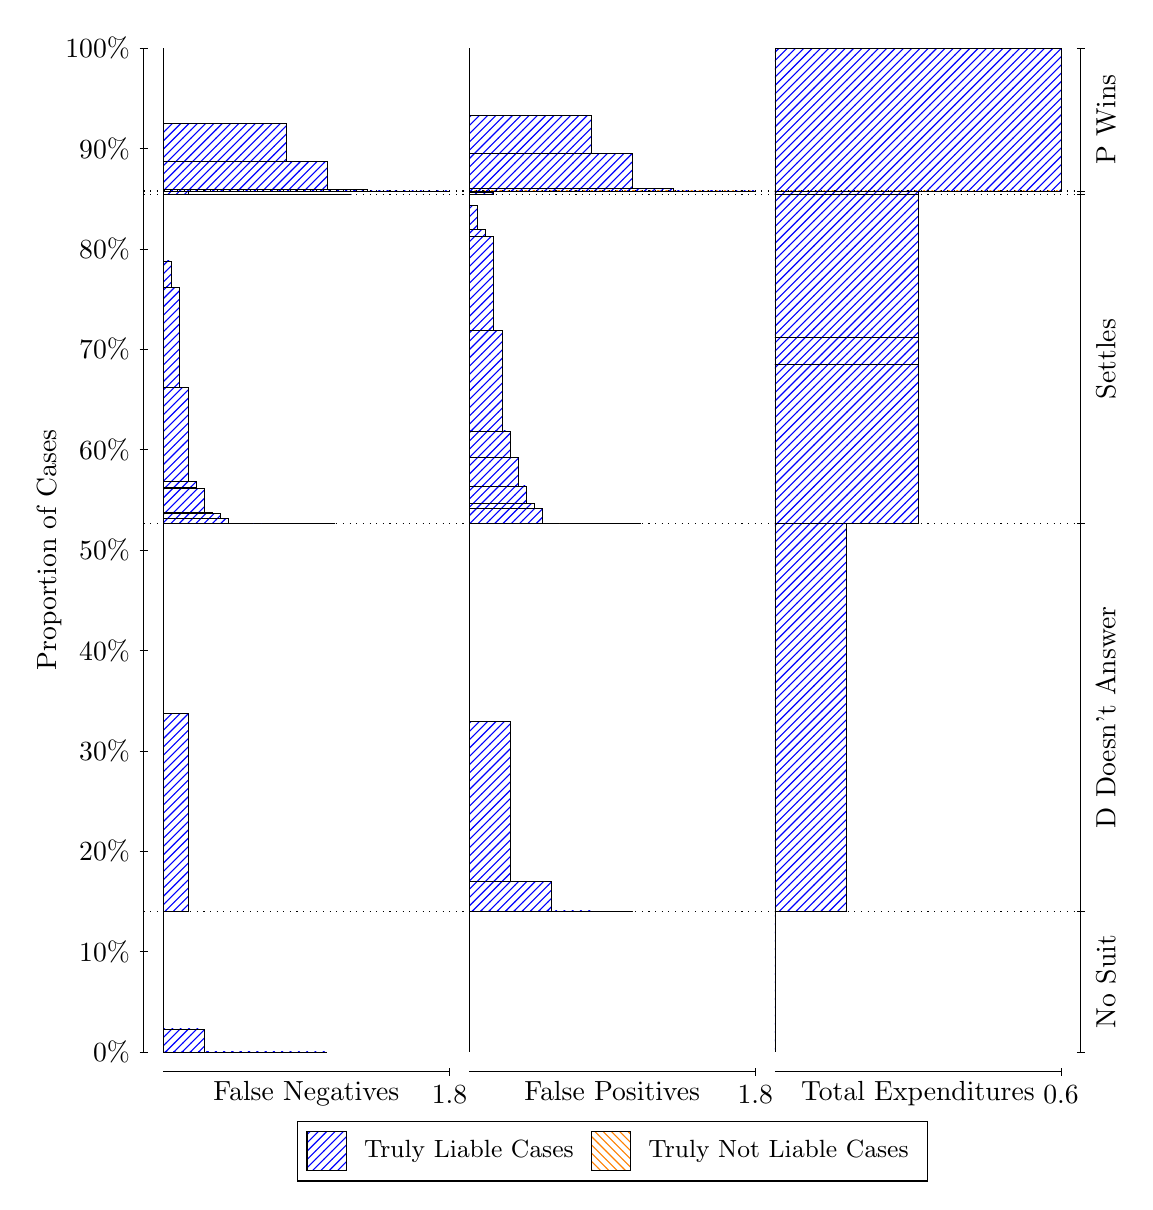
\begin{tikzpicture}
\draw[black, very thin] (1.5,1.75) -- (1.5,14.5);
\node[rotate=90, anchor=center] at (0.3, 8.125) {Proportion of Cases};
\draw[black, very thin] (1.45,1.75) -- (1.55,1.75);
\node[anchor=east] at (1.45, 1.75) {0\%};
\draw[black, very thin] (1.45,3.025) -- (1.55,3.025);
\node[anchor=east] at (1.45, 3.025) {10\%};
\draw[black, very thin] (1.45,4.3) -- (1.55,4.3);
\node[anchor=east] at (1.45, 4.3) {20\%};
\draw[black, very thin] (1.45,5.575) -- (1.55,5.575);
\node[anchor=east] at (1.45, 5.575) {30\%};
\draw[black, very thin] (1.45,6.85) -- (1.55,6.85);
\node[anchor=east] at (1.45, 6.85) {40\%};
\draw[black, very thin] (1.45,8.125) -- (1.55,8.125);
\node[anchor=east] at (1.45, 8.125) {50\%};
\draw[black, very thin] (1.45,9.4) -- (1.55,9.4);
\node[anchor=east] at (1.45, 9.4) {60\%};
\draw[black, very thin] (1.45,10.675) -- (1.55,10.675);
\node[anchor=east] at (1.45, 10.675) {70\%};
\draw[black, very thin] (1.45,11.95) -- (1.55,11.95);
\node[anchor=east] at (1.45, 11.95) {80\%};
\draw[black, very thin] (1.45,13.225) -- (1.55,13.225);
\node[anchor=east] at (1.45, 13.225) {90\%};
\draw[black, very thin] (1.45,14.5) -- (1.55,14.5);
\node[anchor=east] at (1.45, 14.5) {100\%};

\draw[black, very thin] (13.4,1.75) -- (13.4,14.5);
\draw[black, very thin] (13.35,1.75) -- (13.45,1.75);
\node[anchor=west] at (13.35, 1.75) {};
\draw[black, very thin] (13.35,3.5379) -- (13.45,3.5379);
\node[anchor=west] at (13.35, 3.5379) {};
\draw[black, very thin] (13.35,8.459) -- (13.45,8.459);
\node[anchor=west] at (13.35, 8.459) {};
\draw[black, very thin] (13.35,12.64) -- (13.45,12.64);
\node[anchor=west] at (13.35, 12.64) {};
\draw[black, very thin] (13.35,12.675) -- (13.45,12.675);
\node[anchor=west] at (13.35, 12.675) {};
\draw[black, very thin] (13.35,12.686) -- (13.45,12.686);
\node[anchor=west] at (13.35, 12.686) {};
\draw[black, very thin] (13.35,14.5) -- (13.45,14.5);
\node[anchor=west] at (13.35, 14.5) {};

\draw[black, very thin, pattern color=blue, pattern=north east lines] (1.75,1.75) rectangle (3.8262,1.75);
\draw[black, very thin, pattern color=blue, pattern=north east lines] (1.75,1.75) rectangle (3.3071,1.75);
\draw[black, very thin, pattern color=blue, pattern=north east lines] (1.75,1.75) rectangle (2.7881,1.7525);
\draw[black, very thin, pattern color=blue, pattern=north east lines] (1.75,1.7525) rectangle (2.269,2.0427);
\draw[black, very thin, pattern color=orange, pattern=north west lines] (1.75,2.0427) rectangle (1.75,2.0427);
\draw[black, very thin, pattern color=blue, pattern=north east lines] (1.75,2.0427) rectangle (1.75,3.5379);
\draw[black, very thin, pattern color=blue, pattern=north east lines] (1.75,3.5379) rectangle (2.0614,6.0516);
\draw[black, very thin, pattern color=orange, pattern=north west lines] (1.75,6.0516) rectangle (1.75,6.0516);
\draw[black, very thin, pattern color=blue, pattern=north east lines] (1.75,6.0516) rectangle (1.75,8.459);
\draw[black, very thin, pattern color=blue, pattern=north east lines] (1.75,8.459) rectangle (3.93,8.459);
\draw[black, very thin, pattern color=blue, pattern=north east lines] (1.75,8.459) rectangle (3.7224,8.459);
\draw[black, very thin, pattern color=blue, pattern=north east lines] (1.75,8.459) rectangle (3.5148,8.459);
\draw[black, very thin, pattern color=blue, pattern=north east lines] (1.75,8.459) rectangle (3.411,8.459);
\draw[black, very thin, pattern color=blue, pattern=north east lines] (1.75,8.459) rectangle (3.3071,8.459);
\draw[black, very thin, pattern color=blue, pattern=north east lines] (1.75,8.459) rectangle (3.2033,8.459);
\draw[black, very thin, pattern color=blue, pattern=north east lines] (1.75,8.459) rectangle (3.0995,8.459);
\draw[black, very thin, pattern color=blue, pattern=north east lines] (1.75,8.459) rectangle (2.9957,8.459);
\draw[black, very thin, pattern color=blue, pattern=north east lines] (1.75,8.459) rectangle (2.8919,8.459);
\draw[black, very thin, pattern color=blue, pattern=north east lines] (1.75,8.459) rectangle (2.7881,8.4596);
\draw[black, very thin, pattern color=blue, pattern=north east lines] (1.75,8.4596) rectangle (2.6843,8.4596);
\draw[black, very thin, pattern color=blue, pattern=north east lines] (1.75,8.4596) rectangle (2.6843,8.4598);
\draw[black, very thin, pattern color=blue, pattern=north east lines] (1.75,8.4598) rectangle (2.5805,8.5245);
\draw[black, very thin, pattern color=blue, pattern=north east lines] (1.75,8.5245) rectangle (2.4767,8.5885);
\draw[black, very thin, pattern color=blue, pattern=north east lines] (1.75,8.5885) rectangle (2.3729,8.5893);
\draw[black, very thin, pattern color=blue, pattern=north east lines] (1.75,8.5893) rectangle (2.3729,8.6017);
\draw[black, very thin, pattern color=blue, pattern=north east lines] (1.75,8.6017) rectangle (2.269,8.9036);
\draw[black, very thin, pattern color=blue, pattern=north east lines] (1.75,8.9036) rectangle (2.1652,8.9199);
\draw[black, very thin, pattern color=blue, pattern=north east lines] (1.75,8.9199) rectangle (2.1652,8.9958);
\draw[black, very thin, pattern color=blue, pattern=north east lines] (1.75,8.9958) rectangle (2.0614,10.186);
\draw[black, very thin, pattern color=blue, pattern=north east lines] (1.75,10.186) rectangle (1.9576,11.463);
\draw[black, very thin, pattern color=blue, pattern=north east lines] (1.75,11.463) rectangle (1.9576,11.463);
\draw[black, very thin, pattern color=blue, pattern=north east lines] (1.75,11.463) rectangle (1.8538,11.467);
\draw[black, very thin, pattern color=blue, pattern=north east lines] (1.75,11.467) rectangle (1.8538,11.798);
\draw[black, very thin, pattern color=blue, pattern=north east lines] (1.75,11.798) rectangle (1.75,11.798);
\draw[black, very thin, pattern color=orange, pattern=north west lines] (1.75,11.798) rectangle (1.75,11.798);
\draw[black, very thin, pattern color=blue, pattern=north east lines] (1.75,11.798) rectangle (1.75,12.64);
\draw[black, very thin, pattern color=blue, pattern=north east lines] (1.75,12.64) rectangle (4.1376,12.64);
\draw[black, very thin, pattern color=blue, pattern=north east lines] (1.75,12.64) rectangle (3.6186,12.64);
\draw[black, very thin, pattern color=blue, pattern=north east lines] (1.75,12.64) rectangle (3.0995,12.64);
\draw[black, very thin, pattern color=blue, pattern=north east lines] (1.75,12.64) rectangle (2.5805,12.645);
\draw[black, very thin, pattern color=blue, pattern=north east lines] (1.75,12.645) rectangle (2.0614,12.675);
\draw[black, very thin, pattern color=orange, pattern=north west lines] (1.75,12.675) rectangle (1.75,12.675);
\draw[black, very thin, pattern color=blue, pattern=north east lines] (1.75,12.675) rectangle (2.0614,12.677);
\draw[black, very thin, pattern color=orange, pattern=north west lines] (1.75,12.677) rectangle (1.75,12.677);
\draw[black, very thin, pattern color=blue, pattern=north east lines] (1.75,12.677) rectangle (1.75,12.686);
\draw[black, very thin, pattern color=blue, pattern=north east lines] (1.75,12.686) rectangle (5.3833,12.686);
\draw[black, very thin, pattern color=blue, pattern=north east lines] (1.75,12.686) rectangle (4.8643,12.686);
\draw[black, very thin, pattern color=blue, pattern=north east lines] (1.75,12.686) rectangle (4.3452,12.708);
\draw[black, very thin, pattern color=blue, pattern=north east lines] (1.75,12.708) rectangle (3.8262,13.058);
\draw[black, very thin, pattern color=blue, pattern=north east lines] (1.75,13.058) rectangle (3.3071,13.539);
\draw[black, very thin, pattern color=blue, pattern=north east lines] (1.75,13.539) rectangle (2.9957,13.539);
\draw[black, very thin, pattern color=blue, pattern=north east lines] (1.75,13.539) rectangle (2.7881,13.539);
\draw[black, very thin, pattern color=blue, pattern=north east lines] (1.75,13.539) rectangle (2.4767,13.539);
\draw[black, very thin, pattern color=blue, pattern=north east lines] (1.75,13.539) rectangle (2.4767,13.539);
\draw[black, very thin, pattern color=blue, pattern=north east lines] (1.75,13.539) rectangle (2.269,13.539);
\draw[black, very thin, pattern color=blue, pattern=north east lines] (1.75,13.539) rectangle (1.9576,13.543);
\draw[black, very thin, pattern color=blue, pattern=north east lines] (1.75,13.543) rectangle (1.9576,13.544);
\draw[black, very thin, pattern color=orange, pattern=north west lines] (1.75,13.544) rectangle (1.75,13.544);
\draw[black, very thin, pattern color=blue, pattern=north east lines] (1.75,13.544) rectangle (1.75,14.5);
\draw[black, very thin, pattern color=orange, pattern=north west lines] (5.6333,1.75) rectangle (5.6333,1.75);
\draw[black, very thin, pattern color=blue, pattern=north east lines] (5.6333,1.75) rectangle (5.6333,3.5379);
\draw[black, very thin, pattern color=orange, pattern=north west lines] (5.6333,3.5379) rectangle (7.7095,3.5379);
\draw[black, very thin, pattern color=blue, pattern=north east lines] (5.6333,3.5379) rectangle (7.7095,3.5379);
\draw[black, very thin, pattern color=blue, pattern=north east lines] (5.6333,3.5379) rectangle (7.1905,3.5407);
\draw[black, very thin, pattern color=blue, pattern=north east lines] (5.6333,3.5407) rectangle (6.6714,3.9179);
\draw[black, very thin, pattern color=blue, pattern=north east lines] (5.6333,3.9179) rectangle (6.1524,5.9453);
\draw[black, very thin, pattern color=blue, pattern=north east lines] (5.6333,5.9453) rectangle (5.6333,8.459);
\draw[black, very thin, pattern color=orange, pattern=north west lines] (5.6333,8.459) rectangle (7.8133,8.459);
\draw[black, very thin, pattern color=blue, pattern=north east lines] (5.6333,8.459) rectangle (7.8133,8.459);
\draw[black, very thin, pattern color=orange, pattern=north west lines] (5.6333,8.459) rectangle (7.6057,8.459);
\draw[black, very thin, pattern color=blue, pattern=north east lines] (5.6333,8.459) rectangle (7.6057,8.459);
\draw[black, very thin, pattern color=orange, pattern=north west lines] (5.6333,8.459) rectangle (7.3981,8.459);
\draw[black, very thin, pattern color=blue, pattern=north east lines] (5.6333,8.459) rectangle (7.3981,8.459);
\draw[black, very thin, pattern color=blue, pattern=north east lines] (5.6333,8.459) rectangle (7.2943,8.459);
\draw[black, very thin, pattern color=orange, pattern=north west lines] (5.6333,8.459) rectangle (7.1905,8.459);
\draw[black, very thin, pattern color=blue, pattern=north east lines] (5.6333,8.459) rectangle (7.1905,8.459);
\draw[black, very thin, pattern color=blue, pattern=north east lines] (5.6333,8.459) rectangle (7.0867,8.459);
\draw[black, very thin, pattern color=orange, pattern=north west lines] (5.6333,8.459) rectangle (6.9829,8.459);
\draw[black, very thin, pattern color=blue, pattern=north east lines] (5.6333,8.459) rectangle (6.9829,8.459);
\draw[black, very thin, pattern color=blue, pattern=north east lines] (5.6333,8.459) rectangle (6.879,8.4591);
\draw[black, very thin, pattern color=orange, pattern=north west lines] (5.6333,8.4591) rectangle (6.7752,8.4591);
\draw[black, very thin, pattern color=blue, pattern=north east lines] (5.6333,8.4591) rectangle (6.7752,8.4636);
\draw[black, very thin, pattern color=orange, pattern=north west lines] (5.6333,8.4636) rectangle (6.7752,8.4636);
\draw[black, very thin, pattern color=blue, pattern=north east lines] (5.6333,8.4636) rectangle (6.7752,8.4636);
\draw[black, very thin, pattern color=blue, pattern=north east lines] (5.6333,8.4636) rectangle (6.6714,8.4637);
\draw[black, very thin, pattern color=blue, pattern=north east lines] (5.6333,8.4637) rectangle (6.5676,8.4637);
\draw[black, very thin, pattern color=orange, pattern=north west lines] (5.6333,8.4637) rectangle (6.5676,8.4637);
\draw[black, very thin, pattern color=blue, pattern=north east lines] (5.6333,8.4637) rectangle (6.5676,8.6517);
\draw[black, very thin, pattern color=blue, pattern=north east lines] (5.6333,8.6517) rectangle (6.4638,8.7152);
\draw[black, very thin, pattern color=orange, pattern=north west lines] (5.6333,8.7152) rectangle (6.36,8.7152);
\draw[black, very thin, pattern color=blue, pattern=north east lines] (5.6333,8.7152) rectangle (6.36,8.9404);
\draw[black, very thin, pattern color=blue, pattern=north east lines] (5.6333,8.9404) rectangle (6.2562,9.3009);
\draw[black, very thin, pattern color=blue, pattern=north east lines] (5.6333,9.3009) rectangle (6.2562,9.3009);
\draw[black, very thin, pattern color=orange, pattern=north west lines] (5.6333,9.3009) rectangle (6.1524,9.3009);
\draw[black, very thin, pattern color=blue, pattern=north east lines] (5.6333,9.3009) rectangle (6.1524,9.6367);
\draw[black, very thin, pattern color=blue, pattern=north east lines] (5.6333,9.6367) rectangle (6.0486,9.6367);
\draw[black, very thin, pattern color=blue, pattern=north east lines] (5.6333,9.6367) rectangle (6.0486,10.913);
\draw[black, very thin, pattern color=blue, pattern=north east lines] (5.6333,10.913) rectangle (5.9448,12.104);
\draw[black, very thin, pattern color=blue, pattern=north east lines] (5.6333,12.104) rectangle (5.841,12.196);
\draw[black, very thin, pattern color=blue, pattern=north east lines] (5.6333,12.196) rectangle (5.7371,12.498);
\draw[black, very thin, pattern color=blue, pattern=north east lines] (5.6333,12.498) rectangle (5.7371,12.498);
\draw[black, very thin, pattern color=blue, pattern=north east lines] (5.6333,12.498) rectangle (5.6333,12.64);
\draw[black, very thin, pattern color=orange, pattern=north west lines] (5.6333,12.64) rectangle (5.9448,12.64);
\draw[black, very thin, pattern color=blue, pattern=north east lines] (5.6333,12.64) rectangle (5.9448,12.67);
\draw[black, very thin, pattern color=blue, pattern=north east lines] (5.6333,12.67) rectangle (5.6333,12.675);
\draw[black, very thin, pattern color=orange, pattern=north west lines] (5.6333,12.675) rectangle (8.021,12.675);
\draw[black, very thin, pattern color=blue, pattern=north east lines] (5.6333,12.675) rectangle (8.021,12.675);
\draw[black, very thin, pattern color=blue, pattern=north east lines] (5.6333,12.675) rectangle (7.5019,12.675);
\draw[black, very thin, pattern color=blue, pattern=north east lines] (5.6333,12.675) rectangle (6.9829,12.676);
\draw[black, very thin, pattern color=blue, pattern=north east lines] (5.6333,12.676) rectangle (6.4638,12.683);
\draw[black, very thin, pattern color=blue, pattern=north east lines] (5.6333,12.683) rectangle (5.9448,12.686);
\draw[black, very thin, pattern color=orange, pattern=north west lines] (5.6333,12.686) rectangle (9.2667,12.686);
\draw[black, very thin, pattern color=blue, pattern=north east lines] (5.6333,12.686) rectangle (9.2667,12.686);
\draw[black, very thin, pattern color=orange, pattern=north west lines] (5.6333,12.686) rectangle (8.7476,12.686);
\draw[black, very thin, pattern color=blue, pattern=north east lines] (5.6333,12.686) rectangle (8.7476,12.686);
\draw[black, very thin, pattern color=orange, pattern=north west lines] (5.6333,12.686) rectangle (8.2286,12.686);
\draw[black, very thin, pattern color=blue, pattern=north east lines] (5.6333,12.686) rectangle (8.2286,12.721);
\draw[black, very thin, pattern color=orange, pattern=north west lines] (5.6333,12.721) rectangle (7.7095,12.721);
\draw[black, very thin, pattern color=blue, pattern=north east lines] (5.6333,12.721) rectangle (7.7095,13.164);
\draw[black, very thin, pattern color=blue, pattern=north east lines] (5.6333,13.164) rectangle (7.1905,13.642);
\draw[black, very thin, pattern color=blue, pattern=north east lines] (5.6333,13.642) rectangle (6.6714,13.646);
\draw[black, very thin, pattern color=orange, pattern=north west lines] (5.6333,13.646) rectangle (6.36,13.646);
\draw[black, very thin, pattern color=blue, pattern=north east lines] (5.6333,13.646) rectangle (6.36,13.646);
\draw[black, very thin, pattern color=blue, pattern=north east lines] (5.6333,13.646) rectangle (6.1524,13.646);
\draw[black, very thin, pattern color=orange, pattern=north west lines] (5.6333,13.646) rectangle (5.841,13.646);
\draw[black, very thin, pattern color=blue, pattern=north east lines] (5.6333,13.646) rectangle (5.841,13.647);
\draw[black, very thin, pattern color=orange, pattern=north west lines] (5.6333,13.647) rectangle (5.6333,13.647);
\draw[black, very thin, pattern color=blue, pattern=north east lines] (5.6333,13.647) rectangle (5.6333,14.5);
\draw[black, very thin, pattern color=orange, pattern=north west lines] (9.5167,1.75) rectangle (9.5167,1.75);
\draw[black, very thin, pattern color=blue, pattern=north east lines] (9.5167,1.75) rectangle (9.5167,3.5379);
\draw[black, very thin, pattern color=orange, pattern=north west lines] (9.5167,3.5379) rectangle (10.425,3.5379);
\draw[black, very thin, pattern color=blue, pattern=north east lines] (9.5167,3.5379) rectangle (10.425,8.459);
\draw[black, very thin, pattern color=orange, pattern=north west lines] (9.5167,8.459) rectangle (11.333,8.459);
\draw[black, very thin, pattern color=blue, pattern=north east lines] (9.5167,8.459) rectangle (11.333,10.483);
\draw[black, very thin, pattern color=orange, pattern=north west lines] (9.5167,10.483) rectangle (11.333,10.483);
\draw[black, very thin, pattern color=blue, pattern=north east lines] (9.5167,10.483) rectangle (11.333,10.826);
\draw[black, very thin, pattern color=orange, pattern=north west lines] (9.5167,10.826) rectangle (11.333,10.826);
\draw[black, very thin, pattern color=blue, pattern=north east lines] (9.5167,10.826) rectangle (11.333,12.64);
\draw[black, very thin, pattern color=orange, pattern=north west lines] (9.5167,12.64) rectangle (11.333,12.64);
\draw[black, very thin, pattern color=blue, pattern=north east lines] (9.5167,12.64) rectangle (11.333,12.675);
\draw[black, very thin, pattern color=orange, pattern=north west lines] (9.5167,12.675) rectangle (11.333,12.675);
\draw[black, very thin, pattern color=blue, pattern=north east lines] (9.5167,12.675) rectangle (11.333,12.686);
\draw[black, very thin, pattern color=orange, pattern=north west lines] (9.5167,12.686) rectangle (13.15,12.686);
\draw[black, very thin, pattern color=blue, pattern=north east lines] (9.5167,12.686) rectangle (13.15,14.5);
\draw[black, dotted] (1.5,3.5379) -- (13.4,3.5379);
\draw[black, dotted] (1.5,8.459) -- (13.4,8.459);
\draw[black, dotted] (1.5,12.64) -- (13.4,12.64);
\draw[black, dotted] (1.5,12.675) -- (13.4,12.675);
\draw[black, dotted] (1.5,12.686) -- (13.4,12.686);
\draw[black, very thin] (1.75,1.5) -- (5.3833,1.5);
\node[anchor=north] at (3.5667, 1.5) {False Negatives};
\draw[black, very thin] (5.3833,1.45) -- (5.3833,1.55);
\node[anchor=north] at (5.3833, 1.45) {1.8};

\draw[black, very thin] (5.6333,1.5) -- (9.2667,1.5);
\node[anchor=north] at (7.45, 1.5) {False Positives};
\draw[black, very thin] (9.2667,1.45) -- (9.2667,1.55);
\node[anchor=north] at (9.2667, 1.45) {1.8};

\draw[black, very thin] (9.5167,1.5) -- (13.15,1.5);
\node[anchor=north] at (11.333, 1.5) {Total Expenditures};
\draw[black, very thin] (13.15,1.45) -- (13.15,1.55);
\node[anchor=north] at (13.15, 1.45) {0.6};

\node[black, centered, rotate=90] at (13.72, 2.6439) {No Suit};
\node[black, centered, rotate=90] at (13.72, 5.9984) {D Doesn't Answer};
\node[black, centered, rotate=90] at (13.72, 10.55) {Settles};


\node[black, centered, rotate=90] at (13.72, 13.593) {P Wins};

\draw (7.449999999999999,1.5) node[draw=none] (baseCoordinate) {};
\begin{scope}[align=center]
        \matrix[scale=0.5, draw=black, below=0.5cm of baseCoordinate, nodes={draw}, column sep=0.1cm]{
            \node[rectangle, draw, minimum width=0.5cm, minimum height=0.5cm, pattern=north east lines, pattern color=blue] {}; &
            \node[draw=none, font=\small] (B) {Truly Liable Cases}; &
            \node[rectangle, draw, minimum width=0.5cm, minimum height=0.5cm, pattern=north west lines, pattern color=orange] {}; &
            \node[draw=none, font=\small] (B) {Truly Not Liable Cases}; \\
            };
\end{scope}

\end{tikzpicture}
\end{document}